% !TeX program = xelatex
\documentclass[14pt,a4paper,russian]{article}
\usepackage{fontspec}
\usepackage{xunicode,xltxtra} %пакеты для работы xelatex
\usepackage{color}
\setmainfont{Liberation Serif} %выбор шрифта
\usepackage{amsmath}
\usepackage{setspace}
\usepackage{amsmath, amsfonts, amssymb} %математические пактеы
\usepackage{geometry} %разметка страницы
\geometry{
	lmargin=2cm, %левое поле
	rmargin=2cm, %правое поле
	tmargin=2cm, %верхнее поле
	bmargin=2cm, %нижнее поле
	headheight=14pt,
	headsep=1cm,
	footskip=1cm
}

\usepackage{indentfirst} 
\renewcommand{\normalsize}{\fontsize{14pt}{21pt}\selectfont} %установка кегля текста в 14
\usepackage{cancel}
\usepackage{graphics} %пакет для вставки рисунков

\sloppy
\clubpenalty=10000
\widowpenalty=10000

\parindent=1.5cm %абзацный отступ
\linespread{1.2}
\usepackage{longtable} %пакет для работы с такблицами
\usepackage{makecell} %пакет для работы с такблицами
\usepackage{multirow} %пакет для работы с такблицами

\usepackage{caption} %пакте для работы с подписями рисунков и таблиц
\captionsetup[table]{name=Таблицa ,
	position=top, 
	belowskip=0pt,
	aboveskip=0pt,
	format = plain,
	justification=raggedright,
	labelsep=endash}
\captionsetup[figure]{name=Рисунок ,
	position=above,
	belowskip=0pt,
	aboveskip=0pt,
	format = plain,
	justification=raggedright,
	labelsep=endash}

\usepackage{graphicx} %пакет для работы с рисунками
\usepackage{tikz} %пакет для рисования в latex
\usepackage{xcolor} %пакет для работы с цветом
\usepackage{colortbl} %пакет для работы с цветом в таблицах
\usetikzlibrary{arrows} %библиотека для работы со стрелками в рисуемых схемах

\newtheorem{opr}{Определение}[section]
\newtheorem{svva}{Свойства}[opr]
\newtheorem{lem}{Лемма}[section]
\newtheorem{utv}{Утверждение}[section]
\newtheorem{zam}{Замечание}[section]
\newtheorem{teor}{Теорема}[section]
\newtheorem{prim}{Пример}[section]
\newtheorem{sled}{Следствие}[teor]
\newtheorem{zad}{Задача}[section]


\usepackage{titlesec} %пакет для заголовков
\usepackage{tcolorbox} %пакет для работы с цветами

\titleformat{\section}{\fontsize{16pt}{24pt}\selectfont\bfseries}{\thesection.}{.5em}{}
\titleformat{\subsection}{\normalsize\bfseries}{\thesubsection.}{.5em}{}
\titleformat{\subsubsection}{\normalsize\bfseries}{\thesubsubsection.}{.5em}{}

%определение описания нумерованных спсиков
\renewcommand{\labelenumi}{\arabic{enumi})}
\renewcommand{\labelenumii}{\arabic{enumi}.\arabic{enumii})}
\renewcommand{\labelenumiii}{\arabic{enumi}.\arabic{enumii}.\arabic{enumiii})}
\renewcommand{\labelenumiv}{\arabic{enumi}.\arabic{enumii}.\arabic{enumiii}.\arabic{enumiv})}

\usepackage{algorithm} %пакеты для работы с алгоритмами
\usepackage{algpseudocode}

\usepackage{listings}

\lstloadlanguages{C, Python,  [x86masm]{Assembler}}
\usepackage{caption}

\DeclareCaptionFont{white}{\color{white}} %% это сделает текст заголовка белым
%% код ниже нарисует серую рамочку вокруг заголовка кода.
\DeclareCaptionFormat{listing}{\colorbox{gray}{\parbox{\textwidth}{#1#2#3}}}
\captionsetup[lstlisting]{format=listing,labelfont=white,textfont=white}

\usepackage[backend=biber,bibencoding=utf8,maxcitenames=2,style=numeric]{biblatex}

\addbibresource{bibliography/bib.bib}
\newcommand{\anonsection}[1]{\section*{#1}\addcontentsline{toc}{section}{#1}}
\usepackage[unicode=true,colorlinks,filecolor=blue,citecolor=blue,linkcolor=blue]{hyperref}
\newcommand{\N}{\mathbb{N}}
\newcommand{\Z}{\mathbb{Z}}
\newcommand{\Q}{\mathbb{Q}}
\newcommand{\R}{\mathbb{R}}
\renewcommand{\C}{\mathbb{C}}
\lstset{ %
	backgroundcolor=\color{white},   % choose the background color; you must add \usepackage{color} or \usepackage{xcolor}
	basicstyle=\footnotesize,        % the size of the fonts that are used for the code
	breakatwhitespace=false,         % sets if automatic breaks should only happen at whitespace
	breaklines=true,                 % sets automatic line breaking
	captionpos=b,                    % sets the caption-position to bottom
	commentstyle=\color{mygreen},    % comment style
	deletekeywords={...},            % if you want to delete keywords from the given language
	escapeinside={\%*}{*)},          % if you want to add LaTeX within your code
	extendedchars=true,              % lets you use non-ASCII characters; for 8-bits encodings only, does not work with UTF-8
	frame=single,                    % adds a frame around the code
	keepspaces=true,                 % keeps spaces in text, useful for keeping indentation of code (possibly needs columns=flexible)
	keywordstyle=\color{blue},       % keyword style
	language=Octave,                 % the language of the code
	otherkeywords={*,...},           % if you want to add more keywords to the set
	numbers=left,                    % where to put the line-numbers; possible values are (none, left, right)
	numbersep=5pt,                   % how far the line-numbers are from the code
	numberstyle=\tiny\color{mygray}, % the style that is used for the line-numbers
	rulecolor=\color{black},         % if not set, the frame-color may be changed on line-breaks within not-black text (e.g. comments (green here))
	showspaces=false,                % show spaces everywhere adding particular underscores; it overrides 'showstringspaces'
	showstringspaces=false,          % underline spaces within strings only
	showtabs=false,                  % show tabs within strings adding particular underscores
	stepnumber=2,                    % the step between two line-numbers. If it's 1, each line will be numbered
	stringstyle=\color{mymauve},     % string literal style
	tabsize=2,                       % sets default tabsize to 2 spaces
	title=\lstname                   % show the filename of files included with \lstinputlisting; also try caption instead of title
}



\usepackage[notransparent]{svg}
\usepackage{enumerate}
\usepackage{mathtools}
\usepackage[normalem]{ulem}
\begin{document}
%\begin{center}
\thispagestyle{empty} 

\begin{spacing}{1}


\includegraphics[width=35mm]{logo.jpg} 

{

{МИНОБРНАУКИ РОССИИ}

{Федеральное государственное бюджетное образовательное \linebreak учреждение высшего образования}

{
{\bf «МИРЭА – Российский технологический университет» \linebreak РТУ МИРЭА}
}
\rule{1\columnwidth}{1pt}
{Институт кибернетики \smallskip}

{Кафедра информационной безопасности}
\rule{1\columnwidth}{1pt}

}

\end{spacing}

\vspace{1.5cm}

{
КУРСОВАЯ РАБОТА

по дисциплине

<<Методы программирования>>
}

\vspace{0.5cm}

{
Тема курсовой работы

\large\bf
«Название темы»
}

\vspace{1.5cm}

\begin{flushleft}
Студент группы ККСО-00-18: Иванов И.И. \rule{4cm}{0.5pt}

\vspace{1cm}

Руководитель курсовой работы: Кирюхин В.А. \rule{4cm}{0.5pt}

\vspace{1cm}

Работа представлена к защите <<\rule{1cm}{0.5pt}>> \rule{2cm}{0.5pt} 2020 г.

\vspace{1cm}

Допущен к защите <<\rule{1cm}{0.5pt}>> \rule{2cm}{0.5pt} 2020 г.
\end{flushleft}


\vspace{1.5cm}

{Москва 2020}

\end{center}


	\newpage

\renewcommand{\contentsname}{Оглавление}
\setcounter{page}{2}
\tableofcontents

\newpage
\section{Введение}
Рассмотрим общую схему передачи данных по каналу связи:
\begin{figure}[H]
	\centering
	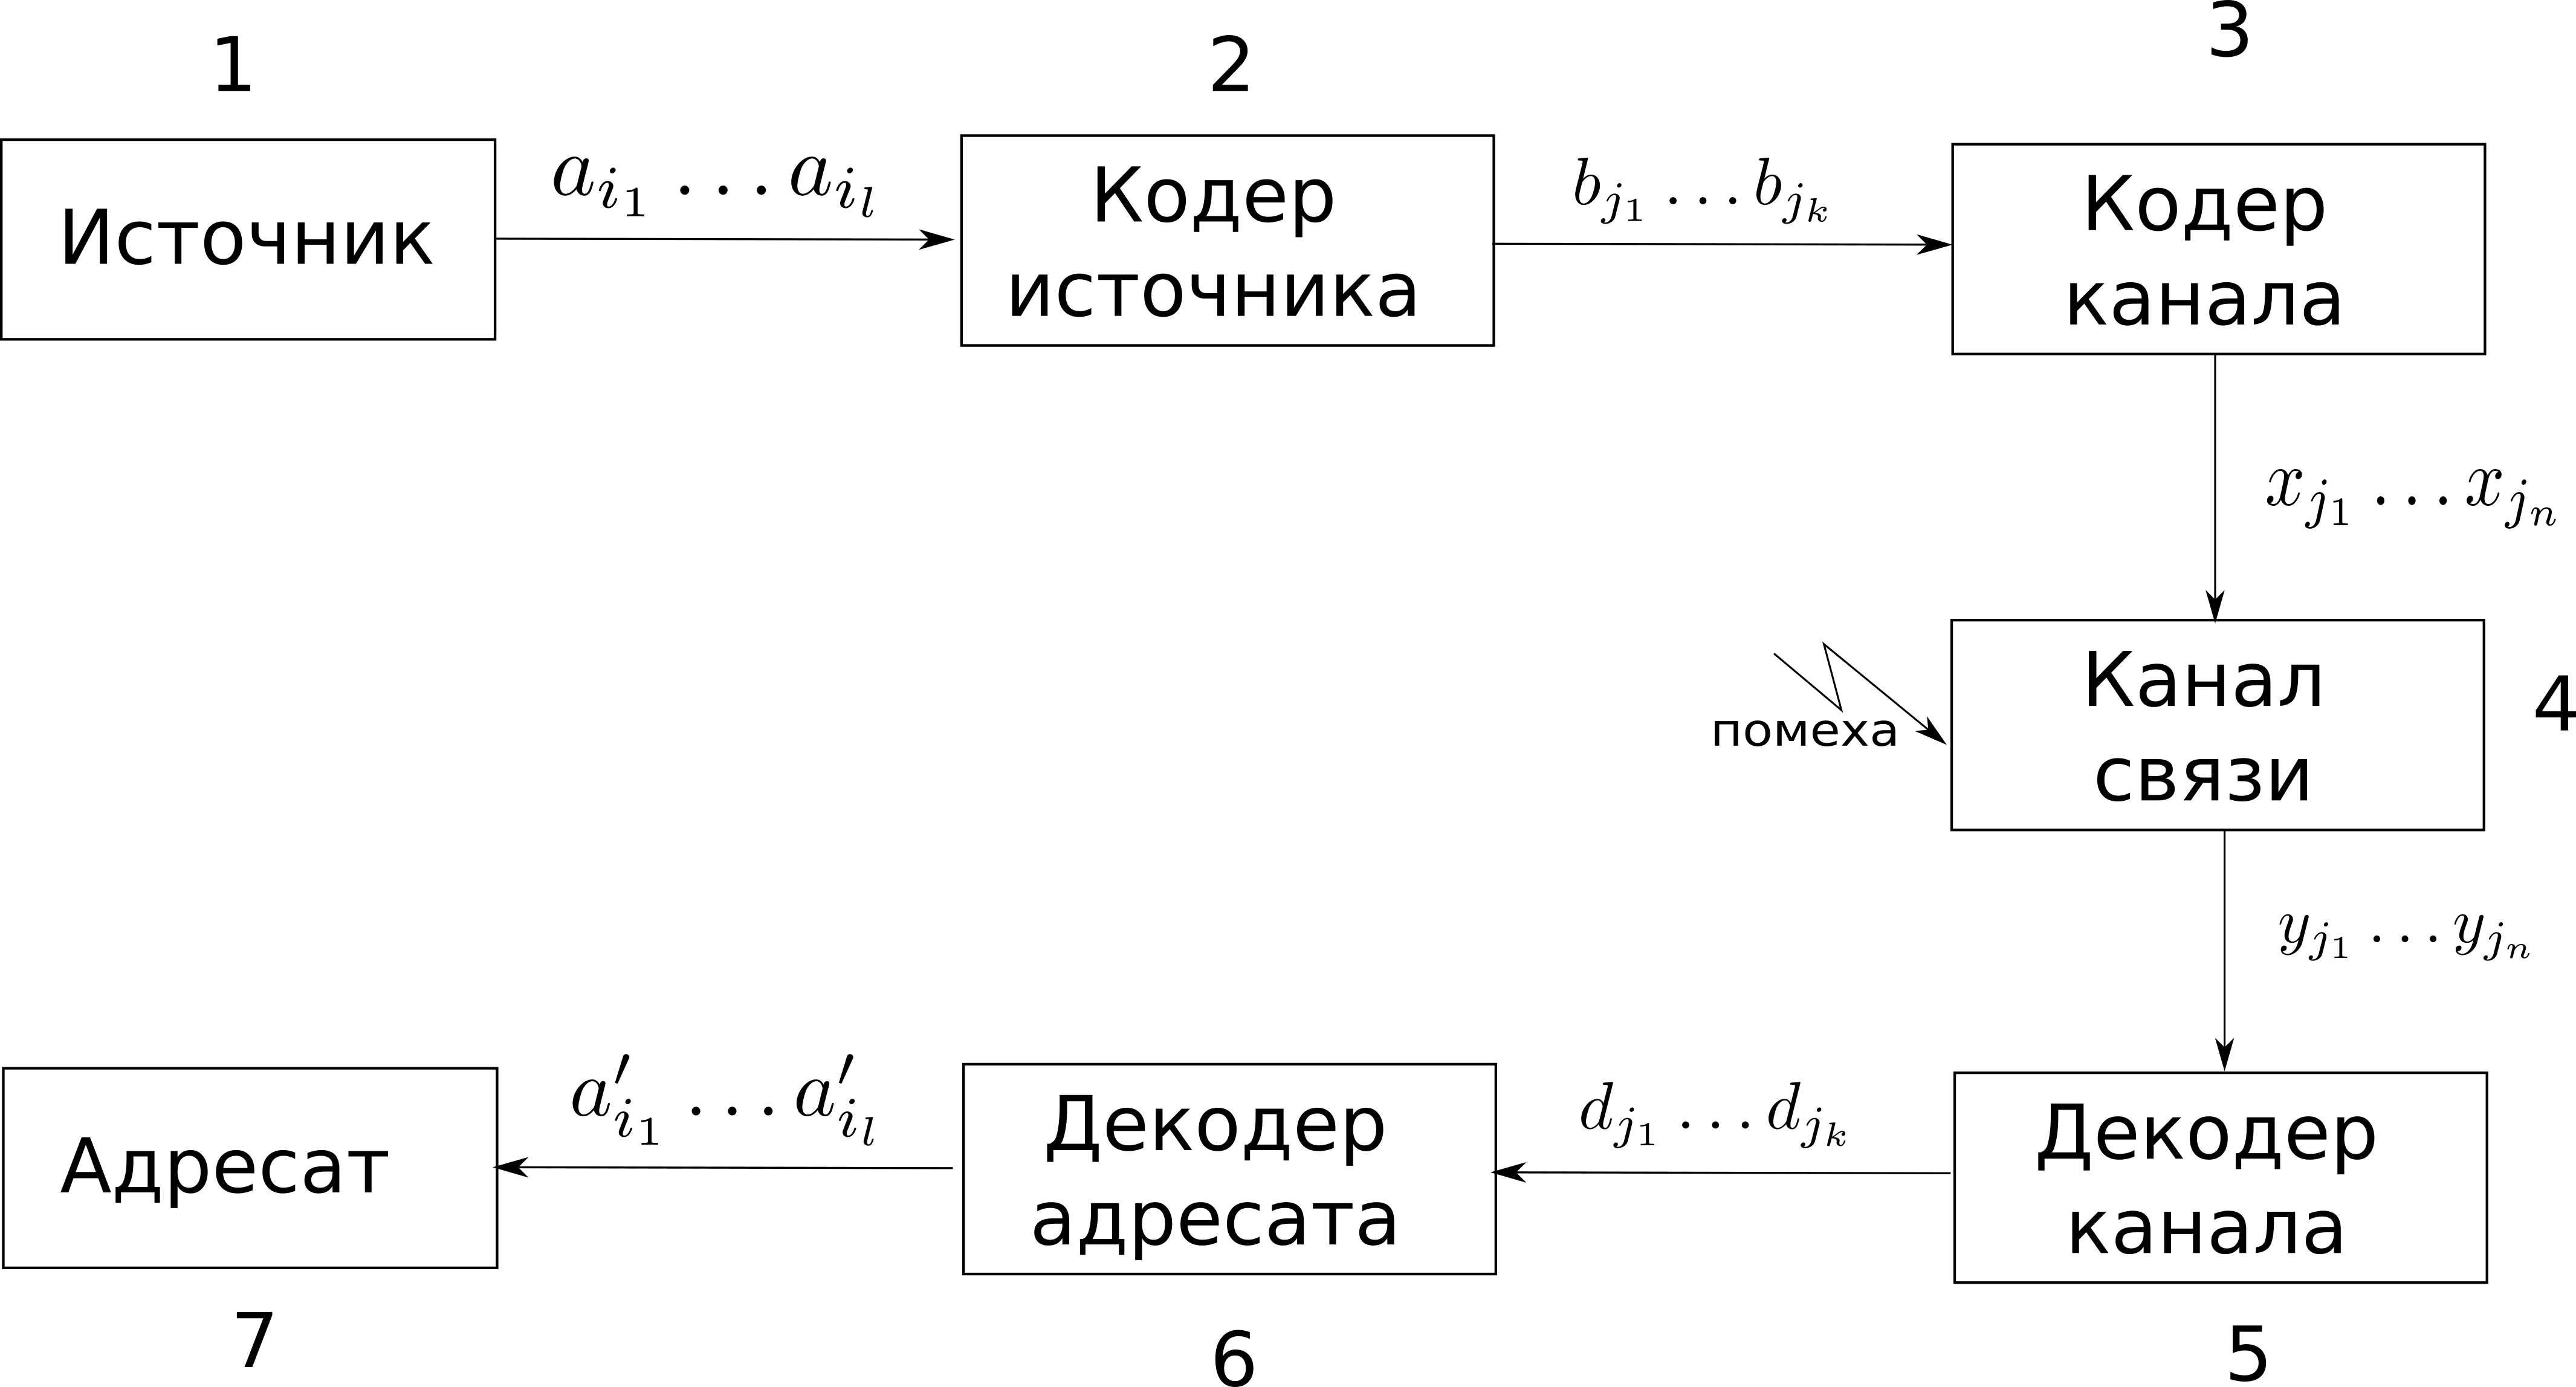
\includegraphics[width=0.7\linewidth]{img/1}
	\caption{Общая схема передачи данных по каналу связи}
	\label{fig:1}
\end{figure}
Задача передачи данных - добиться того, чтобы с вероятностью как можно ближе к 1, выполнилось событие $(a_{i_1} \ldots a_{i_l}) = (a'_{i_1} \ldots a'_{i_l})$. 

Кодер источника (2) предназначен для того, чтобы так преобразовать информацию, порожденную источником, чтобы среднее количество передаваемых символом было минимальным (т.е. решить \uline{задачу оптимального (эффективного) кодирования}). Блок (6) (декодер адресата) осуществляет обратное преобразование.

Блоки 3 и 5 (кодер и декодер канала) решают противоположную задачу: внесение такой избыточности в передаваемое сообщение которое позволит обнаружить и исправить большинство ошибок, которые могут возникнуть в канале связи (природа этих ошибок определяется свойствами среды, в которой существует канал связи) - \uline{это задача помехоустойчивого кодирования}.

В рамках данной курсовой работы, рассматриваются блоки 3 и 5. 
\section{Анализ принципов кодирования/декодирования}
Процесс кодирования это преобразование сообщения из одного алфавита в другой. Процесс декодирования же это обратное преобразование.

Введем определения согласно \cite{Checheta}:

Рассмотрим 2 алфавита: $A = \{a_1, \ldots, a_m\}$ и $B = \{b_1, \ldots, b_D\}$ ($|B| = D$, $|A| = m$)

Введем обозначение: $B^* = \cup_{i=1}^{\infty} B^i$ (т.е. $B^*$ - множество всех возможных слов (любой конечной длинны) состоящих из букв алфавита $B$)

\begin{opr}
	\uline{Алфавитное D-ичное кодирование (кодирующее отображение, код)} - отображение $\varphi: A \rightarrow B^*$ 
	
	При этом $\varphi(a_i) \in B^*$ - называется \uline{кодовым словом}
\end{opr}
\begin{opr}
	Кодирование называется \uline{однозначным}, если отображение $\varphi$ инъективно.
\end{opr}
\begin{opr}
	Кодирование называется \uline{префиксным}, если никакое кодовое слово не является префиксом другого кодового слова.
	
	Кодирование называется \uline{суффиксным}, если никакое кодовое слово не является суффиксом другого кодового слова.
\end{opr}
\begin{teor}
	Если алфавитное кодирование является префиксным или суффиксным, то оно однозначное. Обратное не верно.
\end{teor}

Один из способов графического представления кода - корневое размеченное дерево, в котором каждое ребро помечено каким-либо символом из алфавита $B$, из каждой вершины выходит не более $D$ ребер и каждому кодовому слову однозначно соответствует (существует биекция) лист такой, что последовательность меток ребер пути от корня до листа составляет кодовое слово. 

Например рассмотрим следующий код:
$A \rightarrow B$

$A \rightarrow 0$

$B \rightarrow 10$

$C \rightarrow 11$

Ему будет соответствовать следующее кодовое дерево:
\begin{figure}[H]
	\centering
	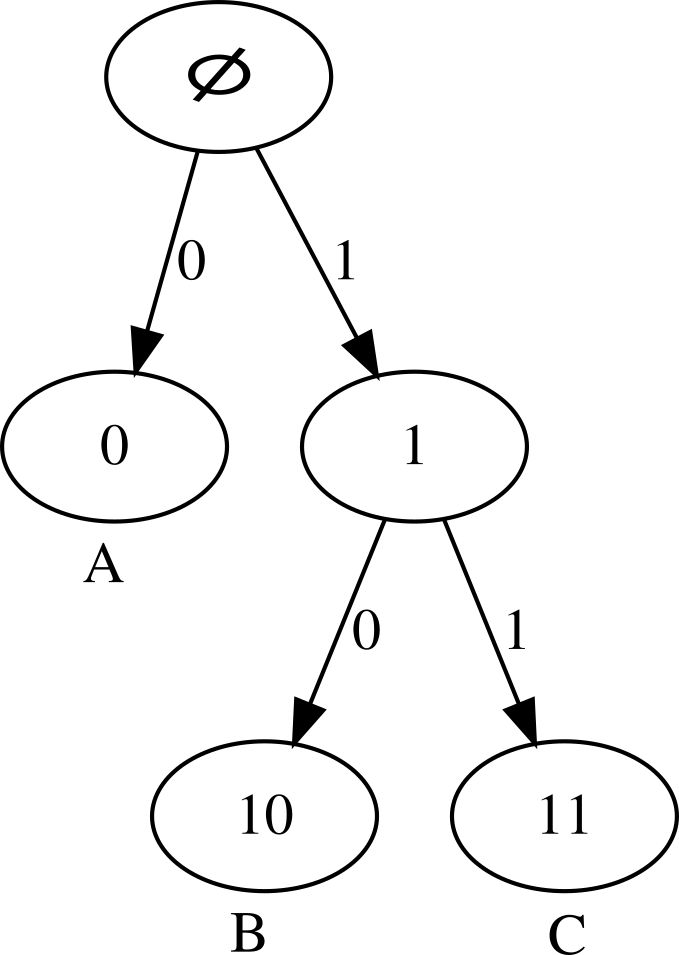
\includegraphics{img/graph}
	\caption{}
	\label{fig:graph}
\end{figure}

\begin{teor}
	\uline{Неравенство-Крафта}
	\begin{enumerate}
		\item Если $\varphi \colon A \rightarrow B^*$ ($|A| = m$) - D-ичное префиксное алфавитное кодирование с длинами кодовых слов $len(\varphi(a_i)) = l_i$, $1 \le i \le m$, то справедливо неравенство
		\begin{equation}
			\sum\limits_{i=1}^{m} D^{-l_i} \le 1 \label{Kraft}
		\end{equation}
		\item Если натуральные числа $D$, $m$, $l_1, \ldots, l_m$ удовлетворяют неравенству \ref{Kraft},то существует D-ичное префиксное алфавитное кодирование $\varphi \colon A \rightarrow B^*$ с длинами кодовых слов $len(\varphi(a_i)) = l_i$, $1 \le i \le m$.
	\end{enumerate}
\end{teor}

Данная теорема позволяет не вдаваясь в подробности какой праобраз в какой образ отображается, проверить может ли вообще существовать однозначный префиксный код при данном наборе длин кодовых слов при данной мощности алфавита $B$. Если неравенство нарушается, то такого однозначного кода точно не существует.
\subsection{Оптимальное (эффективное) кодирование}
Цель оптимального кодирования - так преобразовать текст, чтобы средняя длинна передаваемого сообщения была минимальной.

Пусть $\vec{p} = (p(a_1), \ldots, p(a_m))$, где $p(a_i)$ - вероятность появления буквы $a_i \in A$ . Основная идея оптимального кодирования - сопоставлять буквам с наибольшей вероятностью появления кодовые слова наименьшей длинны.

\begin{opr}
	Пусть заданы алфавит источника $A = \{a_1, \ldots, a_m \}$, кодовый алфавит $B = \{b_1,\ldots, b_D \}$ и распределение $\vec{p} = (p_1, \ldots, p_m)$. Тогда \uline{средней длиной кодового слова} $\varphi \colon A \rightarrow B^*$ называется величина:
	\begin{equation}
		l^\varphi = \sum\limits_{i=1}^m p_i l_i
	\end{equation}
\end{opr}
\begin{opr}
	Алфавитного кодирование $\varphi \colon A \rightarrow B$ называется \uline{оптимальным}, если $\varphi$ однозначно декодируемо и при этом средняя длина $l^\varphi$ минимальна.
\end{opr}
\begin{teor}
	\begin{equation}
		\dfrac{H(\vec{p})}{\log_2 D} \le l^\varphi \le 1 + \dfrac{H(\vec{p})}{\log_2 D}
	\end{equation}
	, где $H(\vec{p}) = H(p(a_1), \ldots, p(a_m)) = H(A) =\sum\limits_{i=1}^m p_i \log_2 \dfrac{1}{p_i}= -\sum\limits_{i=1}^m p_i \log_2 p_i$ - энтропия вероятностной схемы $A$
	$$ A =\begin{pmatrix}
		a_1    & a_2    & \ldots & a_m    \\
		p(a_1) & p(a_2) & \ldots & p(a_m)
	\end{pmatrix}$$ 
\end{teor}
%Рассмотрим некоторые алгоритмы кодирования:
%\subsubsection{Алгоритм Хаффмана}
%Данный алгоритм 
\section{Помехоустойчивое кодирование}
Как было написано ранее задача оптимального кодирования - максимально убрать избыточность кода, чтобы длинна передаваемого сообщения была минимальной. Но при передаче в канале связи могут возникать помехи, а для того чтобы обнаружить и исправить ошибку возникшую в процессе передачи по каналу связи необходимо наоборот внести избыточность в код. В этом заключается суть помехоустойчивого кодирования: внести в код избыточность таким образом, чтобы при возникновении искажений, можно было исправить или по крайней мере обнаружить ошибки возникшие при передаче. При этом желательно, чтобы скорость передачи по каналу связи снизилась как можно меньше, и алгоритмы кодирования/декодирования были оптимальными в смысле трудоемкости по времени и требуемой памяти.

Так же методы при выборе методов кодирования стоит учитывать особенности помех. Например в реальных каналах связи важно соотношение между временем передачи одного символа и средним временем воздействия случайной помехи. Если среднее время воздействия случайной помехи не больше времени передачи одного символа, то стоит выбирать кодирование позволяющее обнаружить и исправить ошибки отдельных символов, а если среднее время воздействия случайной помехи больше времени передачи 1 символа, то нужно такое кодирование, которое позволить корректировать целый набор символов (пакетов ошибок - последовательностей символов, внутри которых имеются ошибки). Так же следует учитывать как именно помехи влияют на передаваемое сообщение: например они могут изменять какой-то символ, удалять какой-то символ или добавлять новый. Так же методы кодирования разделяют на те в которых кодирование очередного символа или блока не зависит от того какой символ или блок кодировался до этого, и те в которых эта зависимость существует.
\section{Блочный код}
Рассмотрим класс блочных(блоковых) кодов.
\begin{opr}
	(Источник: \cite{Checheta})
	
	Пусть даны $k, n \in \N$,  таковы, что $D^k \le q^n$.
	
	\uline{Блоковым кодированием} с входным алфавитом  $B = \{b_1, \ldots, b_D\}$, выходным алфавитом  $X = \{x_1, \ldots, x_q\}$, блоком информационных символов длины $k$ и блоком кодовых символов длины $n$ называется произвольное инъективное отображение $\varphi \colon B^k \rightarrow X^n$.
	
	Множество $\mathcal{C} = \varphi(B^k) \subseteq X^n$ называется блоковым кодом, а его элементы - кодовыми словами.
\end{opr}
Т.е. при использовании блокового кодирования мы берем сообщение произвольной длины, делим его на не пересекающихся части по $k$ символов. Потом каждую часть переводим в алфавит $X$ (на практике часто $X = B$), и добавляем $n-k$ избыточных символов из алфавита $X$. Если длина исходного сообщения не кратна k, то к последнему блоку дописывается такое количество символов из $B$ (каким способом дописывать оговорено заранее и известно как кодеру, так и декодеру) чтобы она стала кратной $k$.

Далее кодовые слова $\mathcal{C}$ последовательно, символ за символом, передаются по каналу связи, в котором могут подвергнутся влиянию помех. И в итоге на вход декодеру поочередно попадает последовательность кодовых слов $y_i^n = (y_{i_1}, \ldots, y_{i_n}) \in Y^n$, которая в следствие виляния помех, может отличатся от последовательности $x_i^n = (x_{i_1}, \ldots, x_{i_n})$ которая была отправлена. Далее задача декодера по последовательности $y_i^n$ восстановить последовательность $x_i^n$ , если произошли ошибки(искажения) исправить, если исправить не удается, то делаем вывод о безуспешной передаче(в таких случаях обычно идет запрос на повторную передачу кодового слова).

( Чаще всего  $B = X = Y = \{0, 1\}$)
\begin{opr}
	(Источник: \cite{Checheta})
	
	\uline{Расстояние Хемминга} на множестве $X^n$ называется отображение $\rho \colon X^n \times X^n \rightarrow \N_0$, задаваемое формулой
	 \begin{equation}
	 	\rho(a^n, b^n) = \sum_{i = 1}^{n} \chi(a_i \ne b_i)
	 \end{equation}
	 где: $a^n \in X^n$, $b^n \in X^n$, $\chi(A)$ - индикатор события A
	 $$\chi(A) = \begin{cases}
	 0, \text{если $A$ - ложь}\\
	 1, \text{если $A$ - истина}
	 \end{cases}$$
\end{opr}
Другими словами $\rho(a^n, b^n)$ это число координат, где $a_i \ne b_i$
\begin{svva} 
	(Источник: \cite{Checheta})
	
	\begin{enumerate}
		\item (неотрицательность) $\rho(a^n, b^n) \ge 0$, причем $\rho(a^n, b^n) = 0 \Rightarrow a^n = b^n$
		\item (cимметричность) $\rho(a^n, b^n) = \rho(b^n, a^n)$
		\item (неравенство треугольника) $\rho(a^n, b^n) + \rho(b^n, c^n) \ge \rho(a^n, c^n)$
	\end{enumerate}
\end{svva}

Если в канал был передан вектор $x_i^n = (x_{i_1}, \ldots, x_{i_n})$ и был получен вектор $y_i^n = (y_{i_1}, \ldots, y_{i_n})$, то говорят, что произошло $\rho(x_i^n, y_i^n) = s$ ошибок.
\newpage

\printbibliography[title={Список использованных источников}]
\addcontentsline{toc}{section}{Список использованных источников}
\end{document}
